%!TEX root = ./template-skripsi.tex
%-------------------------------------------------------------------------------
%                            	BAB IV
%               		KESIMPULAN DAN SARAN
%-------------------------------------------------------------------------------

\chapter{HASIL DAN PEMBAHASAN}

\section{Pemrosesan citra gambar input}
Langkah pertama dalam pemrosesan citra gambar input adalah menentukan rasio piksel 
dari citra tersebut, peneliti mengubah lebar citra menjadi 320 piksel untuk efisiensi 
serta menyamakan ukuran tiap sampel citra gambar, berikut \emph{source code} nya:

\begin{figure}[H]
	\begin{lstlisting}[language=Python, basicstyle=\tiny]
		def setSizeImg(self):
			global new_width, aspect_ratio, new_height
			# set ukuran gambar
			new_width = 320  # Atur ukuran hanya 320 px
			aspect_ratio = self.image.width / self.image.height
			new_height = int(new_width / aspect_ratio)
		
		# Laod image
		self.image = Image.open(self.image_path)

		# Resize ukuran gambar
		self.setSizeImg() 
		self.image = self.image.resize((new_width, new_height)) 
	\end{lstlisting}
	\caption{\emph{source code} mengubah ukuran lebar citra menjadi 320 piksel}
	\label{code:resize_gambar}
\end{figure}

Fungsi \texttt{setSizeImg()} dibuat untuk mengubah ukuran lebar piksel citra 
menjadi 320 piksel, untuk mempertahankan rasionya, maka dibentuk dengan menghitung
menggunakan rumus \texttt{aspect\_ratio} dimana tinggi gambar akan otomatis mengikuti lebar gambar 
dengan perbandingan yang tetap .

\section{Deteksi keliling luka menggunakan \emph{Grabcut}}
Alur deteksi keliling luka menggunakan algoritma \emph{Grabcut} dilakukan melalui
beberapa tahapan, setiap tahapan akan mengolah data input berupa citra gambar luka 
yang disimpan menjadi \emph{array} multidimensi (lebar, tinggi, nilai RGB).
Berikut adalah tahapannya:

\subsection{Inisiasi Kotak Pembatas (\emph{Bounding Box})}

Dalam segmentasi citra luka, dimulai dengan inisiasi kotak atau \emph{bounding box} 
yang digambar mengelilingi area citra luka, berikut \emph{source code} nya:
\begin{figure}[H]
	\begin{lstlisting}[language=Python, basicstyle=\tiny]
		def drawing_rectangle(self):
			print("mulai gambar kotak")
			self.main_canvas.bind("<ButtonPress-1>", self.onClick_rect)
			self.main_canvas.bind("<B1-Motion>", self.onDrag_rect)
			self.main_canvas.bind("<ButtonRelease-1>", self.onRelease_rect)

		def onClick_rect(self, event):
			print("Keberadaan kotak: ",KOTAK["is_drawn"])
			if KOTAK["is_drawn"] is not True:
				KOTAK["titik_start"] = (event.x, event.y)
			else:
				print("kotak sudah ada")

		def onDrag_rect(self, event):
			if KOTAK["is_drawn"] is not True:
				KOTAK["titik_akhir"] = (event.x, event.y)
				self.update_image()

		def onRelease_rect(self, event):
			if KOTAK["titik_start"] and KOTAK["titik_akhir"]:
				KOTAK["coord"] = (self.get_rectangle_coords())
				print("Koordinat Kotak: ", KOTAK["coord"])
				KOTAK["titik_start"] = None
				KOTAK["titik_akhir"] = None
				KOTAK["is_drawn"] = True
			print("Keberadaan kotak: ",KOTAK["is_drawn"])
			print("Koordinat Kotak: ", KOTAK["coord"])

		def get_rectangle_coords(self):
			if KOTAK["titik_start"] and KOTAK["titik_akhir"]:
				x1, y1 = KOTAK["titik_start"]
				x2, y2 = KOTAK["titik_akhir"]
				return (x1, y1, x2, y2)
			else:
				return None

		def drawing_rectangle(self):
			print("mulai gambar kotak")
			self.main_canvas.bind("<ButtonPress-1>", self.onClick_rect)
			self.main_canvas.bind("<B1-Motion>", self.onDrag_rect)
			self.main_canvas.bind("<ButtonRelease-1>", self.onRelease_rect)

	\end{lstlisting}
	\caption{\emph{source code} menggambar kotak pada area luka}
	\label{code:inisiasi_rectangle}
\end{figure}

Ketika kotak sudah tergambar, koordinat dimasukkan kedalam variabel \texttt{KOTAK["coord"]}
pada fungsi \texttt{onRelease\_rect()} yang mana \texttt{KOTAK["coord"]} berupa array 
berisi x1, y1, x2, y2 yang akan digunakan untuk tahap selanjutnya.

\subsection{Inisiasi Piksel}
Tahap selanjutnya adalah membuat salinan \emph{masking} pada citra gambar luka yang diubah
menjadi gambar hitam, salinan dibuat dengan menggunakan \emph{library} \emph{Numpy}
dengan target citra gambar luka. Berikut \emph{source code} nya:

\begin{figure}[H]
	\begin{lstlisting}[language=Python, basicstyle=\tiny]
	self.gambar = np.array(self.image)
	self.gambar2 = self.gambar.copy()
	self.mask = np.zeros(self.gambar2.shape[:2], dtype=np.uint8)
	self.mask2 = self.mask.copy()

	def inisiasi_piksel(self):
		self.alpha[self.rect[1]:self.rect[1] + self.rect[3],self.rect[0]:self.rect[0] + self.rect[2]] = F_TF
		self.trimap['TB'] = np.where(self.alpha == F_TB)
		self.trimap['TU'] = np.where(self.alpha == F_TF)
		"""Inisiasi GMM"""
		self.gmm_fg =  MixtureModel(self.trimap['TU'], 
						self.gambar[self.trimap['TU']], 
						self.komponen_gmm, self.theta['TU'])
		self.gmm_bg =  MixtureModel(self.trimap['TB'], 
						self.gambar[self.trimap['TB']], 
						self.komponen_gmm, self.theta['TB'])
		self.gmm_fg.init_gmm_rand(self.gambar[self.trimap['TU']], self.theta['TU'])
		self.gmm_bg.init_gmm_rand(self.gambar[self.trimap['TB']], self.theta['TB'])
	\end{lstlisting}
	\caption{\emph{source code} inisasi objek gmm \emph{foreground} dan \emph{background} }
	\label{code:mask_image}
\end{figure}

Variabel  \texttt{self.gmm\_fg} dan \texttt{self.gmm\_bg} dibuat sebagai penanda antara objek untuk
\emph{foreground} dan \emph{background}, masing masing memiliki parameter \texttt{self.gambar}, 
\texttt{self.theta}, \texttt{self.trimap}, dan \texttt{self.komponen\_gmm}. Parameter 
tersebut dibedakan nilainya yakni \textbf{'TU'} atau \textbf{'TB'}. 

\begin{figure}[H]
	\begin{lstlisting}[language=Python, basicstyle=\tiny]
	def init_gmm_rand(self, z, theta):
        labels_k = []
        for i in range(z.shape[0]):
            labels_k.append(random.randint(0, self.komponen_gmm-1))
        labels_k = np.array(labels_k)
        self.count_params(z, labels_k, theta)
	\end{lstlisting}
	\caption{\emph{source code} menentukan label awal secara acak}
	\label{code:init_gmm_random}
\end{figure}

Fungsi \texttt{init\_gmm\_rand()} memiliki tugas sebagai pembuat label gmm secara 
acak sepanjang  \texttt{self.gambar} dengan batas angka yakni dari angka 0 sampai 
\texttt{self.komponen\_gmm}, setelah label terbentuk dilanjutkan dengan menjalankan 
fungsi \texttt{count\_params} untuk menghitung nilai GMM berdasarkan nilai awal 
(inisiasi). Berikut \emph{source code} nya:

\subsection{Menentukan Komponen Awal GMM}
Tahap ini merupakan tahap pertama pada gambar \ref{img:segmentasi_grabcut}. Setelah
membuat variabel gmm (fg dan bg) didalamnya terdapat fungsi untuk menentukan dan 
menghitung komponen gmm awal. Berikut \emph{source code} nya:

\begin{figure}[H]
	\begin{lstlisting}[language=Python, basicstyle=\tiny]
	def assign_gmm(self):
        """Step 1 (assign GMM) pada gambar 2.11"""
        print('\nMulai assign GMM')
        self.komponen_piksel[self.trimap['TU']] = self.gmm_fg.assign_component(
            self.gambar[self.trimap['TU']], self.theta['TU'], self.komponen_gmm
        )
        self.komponen_piksel[self.trimap['TB']] = self.gmm_bg.assign_component(
            self.gambar[self.trimap['TB']], self.theta['TB'], self.komponen_gmm
        )
	\end{lstlisting}
	\caption{\emph{source code} menghitung nilai gmm menggunakan label awal}
	\label{code:assign_gmm}
\end{figure}

Fungsi \texttt{assign\_component} adalah fungsi yang menghitung nilai akumulasi 
dari distribusi probabilitas gaussian yang terdapat pada gambar \ref{img:segmentasi_grabcut}
tahap pertama. Berikut \emph{source code} nya:

\begin{figure}[H]
	\begin{lstlisting}[language=Python, basicstyle=\tiny]
	def assign_component(self, z, theta, komponen_gmm):
        gauss_distribution = []
        for k in range(komponen_gmm):
            gauss_score = self.dis_mult(z, k, theta)
            gauss_distribution.append(gauss_score)
        gauss_distribution = np.array(gauss_distribution)
        gauss_distribution = gauss_distribution.T

        return np.argmin(gauss_distribution, axis=1)
	\end{lstlisting}
	\caption{\emph{source code} menghitung akumulasi distribusi gaussian}
	\label{code:assign_component}
\end{figure}

Hasil dari tahap ini adalah label gmm yang telah dihitung yang kemudian akan dipakai 
di tahap selanjutnya.


\subsection{Mempelajari Parameter GMM}
Masuk ke tahap selanjutnya (kedua) dari gambar \ref{img:segmentasi_grabcut} dimana 
label gmm yang sudah diperbarui akan digunakan untuk menghitung kembali parameter 
gmm yakni \texttt{self.theta}. Berikut \emph{source code} nya:

\begin{figure}[H]
	\begin{lstlisting}[language=Python, basicstyle=\tiny]
	def mempelajari_gmm(self):
        self.gmm_fg.count_params(self.gambar[self.trimap['TU']], 
                                 self.komponen_piksel[self.trimap['TU']], 
                                 self.theta['TU'])

        self.gmm_bg.count_params(self.gambar[self.trimap['TB']], 
                                 self.komponen_piksel[self.trimap['TB']], 
                                 self.theta['TB'])

        idx_TU = np.where(self.alpha.reshape(-1) == F_TF)

		self.D_count_fg = []
        self.D_count_bg = []
        for kn in range(self.komponen_gmm):
            zn = self.gambar.reshape(-1, 3)[idx_TU]

            tmp_d_fg = self.gmm_fg.d_calc(zn, kn, self.theta['TU'])
            tmp_d_bg = self.gmm_bg.d_calc(zn, kn, self.theta['TB'])

            self.D_count_fg.append(tmp_d_fg)
            self.D_count_bg.append(tmp_d_bg)

        self.D_count_fg = np.array(self.D_count_fg)
        self.D_count_bg = np.array(self.D_count_bg)
        self.U_count_fg = np.sum(self.D_count_fg, axis=0)
        self.U_count_bg = np.sum(self.D_count_bg, axis=0)       
	\end{lstlisting}
	\caption{\emph{source code} mempelajari parameter GMM}
	\label{code:learn_gmm}
\end{figure}

Setelah mendapat parameter gmm yang baru, selanjutnya adalah menghitung nilai \(D\)
dengan menggunakan rumus \ref{eq:rumus_D}, fungsi yang menghitungnya terdapat pada 
fungsi \texttt{d\_calc}. Berikut \emph{source code} nya:

\begin{figure}[H]
	\begin{lstlisting}[language=Python, basicstyle=\tiny]
	def d_calc(self, zn, kn, theta):
        gauss_res1 = self.gauss_dist_second(zn, kn, theta)
        d_res1 = -np.log(theta['koefisien'][kn]) + gauss_res1

        return d_res1
	\end{lstlisting}
	\caption{\emph{source code} menghitung nilai D}
	\label{code:count_d}
\end{figure}

\subsection{Segmentasi Gambar dengan Algoritma \emph{Mincut}}
Tahap terakhir adalah segmentasi gambar dengan algoritma \emph{mincut}, tahap 
ini bertujuan untuk melakukan pemotongan gambar yang telah dikalkulasi pada 
tahap sebelumnya, algoritma ini membutuhkan adanya graf yang dibuat dari gambar 
citra, \emph{node} pada graf merepresentasikan piksel dalam citra. 
Berikut \emph{source code} nya:

\begin{figure}[H]
	\begin{lstlisting}[language=Python, basicstyle=\tiny]
	def build_graph(self):
		self.gc_graph = ig.Graph(self.kolom * self.baris + 1)
		self.gc_graph.add_edges(self.edges)
	\end{lstlisting}
	\caption{\emph{source code} Membangun graf}
	\label{code:build_graph}
\end{figure}

Setelah graf terbentuk, segmentasi akan dilakukan dengan algoritma \emph{mincut}.
Berikut \emph{source code} nya:
\begin{figure}[H]
	\begin{lstlisting}[language=Python, basicstyle=\tiny]
	def mincut_segmentation(self):

        mincut = self.gc_graph.st_mincut(
        self.source_gc, self.sink_gc, self.kapasitas_graph)

        idx_pr = np.where(self.alpha == F_TF)
        img_indexes = np.arange(self.baris * self.kolom,
                                dtype=np.uint32).reshape(self.baris, self.kolom)

        self.alpha[idx_pr] = np.where(np.isin(img_indexes[idx_pr], mincut.partition[0]),F_TF, F_TB)
	\end{lstlisting}
	\caption{\emph{source code} Membangun graf}
	\label{code:mincut_segmentation}
\end{figure}



\section{Eksperimen}
\emph{Source code} program disimpan di dalam repositori yang dapat diakses di
\url{https://github.com/DragonFly378/Skripsi_Hafiz} di bawah lisensi \emph{GNU General Public License v3.0.}
Rancangan eksperimen deteksi keliling luka dengan algoritma \emph{Grabcut}. Proses 
ini diperlukan adanya penyesuaian parameter dari algoritma yang dijalankan dengan 
data yang tersedia untuk setiap citra. Setelah hasil segmentasi citra didapatkan,
dilanjutkan dengan identifikasi citra hasil segmentasi dan dibandingkan terhadap area 
\emph{ground truth} untuk kemudian dihitung akurasinya menggunakan persamaan \ref{eq:validasi}.
Rincian lengkap hasil dari parameter dan validasi citra tersedia di bagian \textbf{lampiran C}.

\begin{figure}[H]
	\centering
	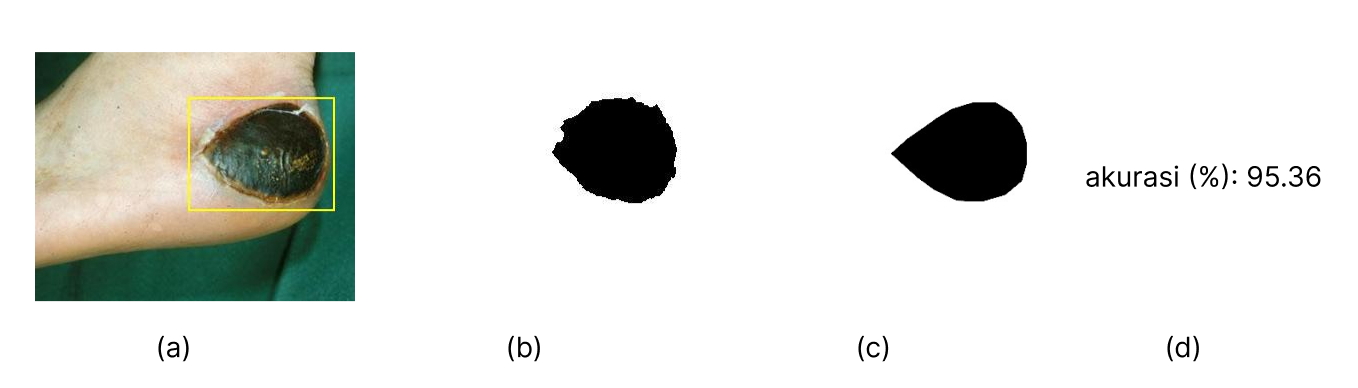
\includegraphics[width=0.8\textwidth]{gambar/hasil_bab4.jpg}
	\caption{(a) Kotak pembatas (b) Hasil segmentasi (c) Area \emph{ground truth} (d) Akurasi}
	\label{img:hasil_segmentasi}
\end{figure}

\section{Analisa hasil}
Berikut analisa hasil setelah melakukan eksperimen terhadap populasi:
\begin{enumerate}
	\item Hasil dari deteksi keliling luka menggunakan algoritma \emph{GrabCut} 
	kategori luka hitam menghasilkan 24 data yang area segmentasi akhirnya memiliki 
	nilai akurasi rata-rata 91.5\%.

	\item Hasil dari deteksi keliling luka menggunakan algoritma \emph{GrabCut} 
	kategori luka kuning menghasilkan 14 (dari 15 data) yang area segmentasi akhirnya 
	memiliki nilai akurasi rata-rata 82.7\%.

	\item Hasil dari deteksi keliling luka menggunakan algoritma \emph{GrabCut} 
	kategori luka merah menghasilkan 33 data yang area segmentasi akhirnya memiliki 
	nilai akurasi rata-rata 93.8\%.

	% \item Hasil dari deteksi keliling luka menggunakan \emph{snake} versi integer 
	% kategori luka hitam yang dilakukan oleh \cite{Rizki:2022} menghasilkan 5 data 
	% (dari 24 data) yang area segmentasi akhirnya memiliki nilai akurasi rata-rata 
	% 84.18\% sedangkan deteksi keliling luka menggunakan \emph{Grabcut} kategori 
	% luka hitam memiliki nilai akurasi rata-rata 92.57\%.

	% \item Hasil dari deteksi keliling luka menggunakan \emph{snake} versi integer 
	% kategori luka kuning yang dilakukan oleh \cite{Rizki:2022} menghasilkan 5 data 
	% (dari 15 data) yang area segmentasi akhirnya memiliki nilai akurasi rata-rata 
	% 76.14\% sedangkan deteksi keliling luka menggunakan \emph{Grabcut} kategori 
	% luka kuning memiliki nilai akurasi rata-rata 66.1\%.

	% \item Hasil dari deteksi keliling luka menggunakan \emph{snake} versi integer 
	% kategori luka merah yang dilakukan oleh \cite{Rizki:2022} menghasilkan 2 data 
	% (dari 32 data) yang area segmentasi akhirnya memiliki nilai akurasi rata-rata 
	% 62.25\% sedangkan deteksi keliling luka menggunakan \emph{Grabcut} kategori 
	% luka merah memiliki nilai akurasi rata-rata 95.74\%.

	% \item Hasil dari deteksi keliling luka menggunakan \emph{snake} versi interpolasi 
	% kategori luka hitam yang dilakukan oleh \cite{Rizki:2022} menghasilkan 21 data 
	% (dari 24 data) yang area segmentasi akhirnya memiliki nilai akurasi rata-rata 
	% 87.63\% sedangkan deteksi keliling luka menggunakan \emph{Grabcut} kategori 
	% luka hitam memiliki nilai akurasi rata-rata 91.94\%.

	% \item Hasil dari deteksi keliling luka menggunakan \emph{snake} versi interpolasi 
	% kategori luka kuning yang dilakukan oleh \cite{Rizki:2022} menghasilkan 11 data 
	% (dari 15 data) yang area segmentasi akhirnya memiliki nilai akurasi rata-rata 
	% 79.21\% sedangkan deteksi keliling luka menggunakan \emph{Grabcut} kategori 
	% luka kuning memiliki nilai akurasi rata-rata 80.45\%.

	% \item Hasil dari deteksi keliling luka menggunakan \emph{snake} versi interpolasi 
	% kategori luka merah yang dilakukan oleh \cite{Rizki:2022} menghasilkan 12 data 
	% (dari 32 data) yang area segmentasi akhirnya memiliki nilai akurasi rata-rata 
	% 89.73\% sedangkan deteksi keliling luka menggunakan \emph{Grabcut} kategori 
	% luka merah memiliki nilai akurasi rata-rata 93.31\%.

	\item Hasil dari deteksi keliling luka menggunakan algoritma \emph{GrabCut} 
	untuk semua kategori menghasilkan 70 (dari 71 data) yang area segmentasi akhirnya 
	memiliki nilai akurasi rata-rata 89.36\%.

\end{enumerate}

% Baris ini digunakan untuk memban tu dalam melakukan sitasi
% Karena diapit dengan comment, maka baris ini akan diabaikan
% oleh compiler LaTeX.
\begin{comment}
\bibliography{daftar-pustaka}
\end{comment}